\documentclass{article}
\usepackage[utf8]{inputenc}
\usepackage{graphicx}
%\usepackage{pgfgantt}

\title{Programmation visuelle de r\'eseaux neuronaux profonds \\ Cahier des besoins}
\author{ALLIO Luc & CHATELAIN Virgile & PELLEGRINI Charles & TSIAPKOLIS Panagiotis}
\date{01 Février 2018}

\begin{document}

\maketitle

\section{Introduction}

L'apprentissage profond (\textit{deep learning} en anglais) est une méthode d'apprentissage automatique reposant sur la simulation de multiples couches de neurones par des transformations mathématiques. C'est une méthode qui se développe beaucoup dernièrement : en effet, cette approche est de plus en plus utilisée pour la création d'intelligences artificielles. \\

Le deep learning est utilisé dans de très nombreux secteurs, aussi variés que la sécurité informatique (par exemple, la société \textit{Tehtris} exploite l'apprentissage profond avec leur solution logicielle, \textit{eGambit}\cite{eGambit2017}, afin de détecter les malwares non connus), la médecine (pour la détection de carcinomes\cite{Cruz-Roa2013} par exemple) ou la finance (pour les problèmes de prédiction et de classification financière\cite{DLFinance}). \\

Il existe à l'heure actuelle de nombreuses solutions pour manipuler des réseaux de neurones profonds. Parmi les plus populaires, on trouve \textit{TensorFlow}\cite{MartinAbadi2015} de Google, \textit{Caffe}\cite{YangqingJia2014}, ou encore \textit{Keras}\cite{chollet2015keras} qui est une sur-couche d'autres solutions telles que \textit{TensorFlow} ou \textit{CNTK}\cite{Microsoft2015}, développé par Microsoft. Ces solutions proposent toutes une interface de programmation principalement disponible pour le langage \textit{Python} afin de décrire les transformations mathématiques qui seront appliquées aux données.\\


D'autre part, il existe certaines solutions pour faire de la programmation visuelle en blocs, c'est à dire programmer en assemblant des blocs de bas niveau ayant chacun un rôle, comme une condition, un type de données et des paramètres, etc. Ainsi, l'utilisateur peut créer un programme sans connaissances préalables dans un quelconque langage. Par exemple, \textit{Blockly}\cite{ErikPasternak2017} de Google, ou encore \textit{Scratch}, principalement destiné aux enfants et qui a plutôt un rôle éducatif. \\

On peut aussi noter qu'il n'y a pas encore de format ouvert qui a su s'imposer pour permettre aux différents outils d'apprentissage profond existants de partager leurs fichiers : par exemple, le standard ouvert \textit{ONNX}\cite{onnx2017} conçu pour représenter des modèles d'apprentissage profond, bien que supporté par de nombreux partenaires parmi lesquels \textit{Amazon}, \textit{Facebook} et \textit{Microsoft}, n'est pas encore adopté par \textit{Keras}. Un des contributeurs du projet a d'ailleurs explicité son point de vue sur la question : pour lui, le support de ces formats externes n'est pas intéressant tant qu'ils n'implémentent pas de fonctionnalités innovantes ou qu'ils n'ont pas été adoptés par un nombre conséquent d'utilisateurs\cite{cholletsavage}. D'autres solutions, comme \textit{NNEF}\cite{nnef2017} ou \textit{OpenVX}\cite{openvx2017}, sont proposées par le consortium \textit{Khronos}.\\

Cependant, à notre connaissance, il est pour le moment impossible de créer un réseau de neurones artificiel sans écrire de code, ce qui rend leur création peu accessible à ceux qui ne maîtrisent pas la programmation. \smallbreak

Le projet consiste donc en la programmation d’une interface permettant la création de réseaux neuronaux profonds sous forme de graphe, chaque noeud représentant un traitement et chaque arête les données transformées (des images, du son par exemple). Le logiciel devra coder le réseau neuronal à partir du graphe, et le renvoyer à l'utilisateur.
Ce logiciel permettrait aux utilisateurs dont la programmation n'est pas le cœur de métier de créer des réseaux neuronaux plus aisément.

\subsection{Diagramme de cas d'utilisation}

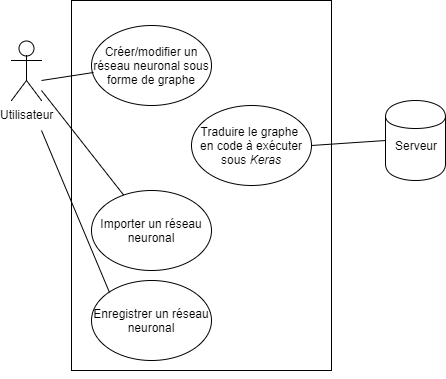
\includegraphics{UseCasePDP.png}

\section{Description des besoins}
\subsection{Besoins fonctionnels}

Le programme doit donc être composé d'une interface graphique accessible par navigateur web, qui permettra à l'utilisateur de créer des graphes représentant des réseaux de neurones profonds, puis d'envoyer un modèle contenant les informations du graphe à un serveur. Ce dernier aura pour rôle la création d'un code exploitable par \textit{Keras} à partir du fichier reçu, qu'il devra renvoyer à l'utilisateur. \smallbreak

\subsubsection{Côté client}

Le client aura donc accès à une interface graphique composée d'une zone centrale où il visualisera le graphe, d'une barre d'outil permettant entre autre d'enregistrer/charger des graphes ou encore d'utiliser la fonction zoom, ainsi que de deux panneaux latéraux, l'un pour choisir les transformations à ajouter au graphe (sous forme de noeuds), l'autre pour modifier les paramètres de cette transformation. \\

L'utilisateur doit pouvoir:
\begin{itemize}
    \item Afficher l'interface web via son navigateur (Priorité : haute)
    \item Visualiser le graphe d'apprentissage (Priorité : haute) \\
          Un graphe étant composé:
        \begin{itemize}
            \item D'une entrée initiale (les données à traiter)
            \item De noeuds représentant les traitements, qui auront une apparence graphique spécifique à la transformation associée. Les noeuds peuvent avoir une ou plusieurs entrées et sorties depuis et vers d'autres noeuds.
            \item D'arêtes, représentant les données transitant entre chaque transformation.
            \item D'une sortie finale (le résultat des traitements)
        \end{itemize}
    \item Visualiser un espace de sélection des traitements ajoutables au graphe (Priorité : haute)
        \begin{itemize}
            \item Les traitements seront affichés dans cet espace sous la même forme que dans l'espace d'affichage.
            \item Il sera possible d'ajouter un traitement via glisser/déposer depuis l'espace de sélection vers la zone d'affichage du graphe.
        \end{itemize}
    \item Modifier les paramètres de chaque traitement via le panneau latéral (Priorité : haute)
    \item Supprimer des traitements du graphe (Priorité : haute)
    \item Déplacer des éléments du graphe dans l'espace de visualisation avec la souris (Priorité : moyenne) \\
            Cela revient à pouvoir: 
        \begin{itemize}
            \item Déplacer les noeuds 
            \item Modifier les trajectoires des arêtes
            \item Modifier les points d'attache des arêtes
        \end{itemize}
    \item Créer des groupes de traitements lorsque ceux-ci se répètent dans le panneau latéral de sélection des traitements (Priorité : basse)
    \item Enregistrer un graphe sur sa machine via la barre d'outil (Priorité : moyenne)
    \item Importer des scripts pour les afficher sous forme de graphe via la barre d'outil (Priorité : basse)
    \item Demander au serveur de créer le code correspondant au graphe affiché (Priorité : haute)
    \item Utiliser une fonction de zoom sur le graphe via la barre d'outil (Priorité : basse)
\end{itemize}


\subsubsection{Côté serveur}

\begin{itemize}
    \item Le serveur doit pouvoir récupérer le graphe du client et renvoyer un ficher exploitable via \textit{Keras}. (Priorité : haute)
    \item Éventuellement exécuter le script sur le serveur (Priorité : basse)
\end{itemize}

\subsection{Besoins non-fonctionnels}
\subsubsection{Portabilité}
\begin{itemize}
\item La partie client doit fonctionner sur les navigateurs les plus utilisés du marché, notamment \textit{Mozilla Firefox} version supérieure à 57, \textit{Google Chrome} version supérieure à 63, et \textit{Apple Safari} version supérieure à 11.
\item La partie serveur doit fonctionner dans un conteneur \textit{Docker}\cite{Fink2014} utilisable à partir de la version 17.
\end{itemize}
%\subsubsection{Performances}
%\begin{itemize}
%\item L'empreinte mémoire du client ne doit pas dépasser 2 Go de mémoire.
% La phase de test pour assurer ce besoin consiste à tester le programme de manière itérative sur des machines virtuelles dont les performances sont progressivement diminuées 

%\end{itemize}
\subsubsection{Extensibilité}
\begin{itemize}
\item En cas d'ajout de nouveaux types de layers dans \textit{Keras}, il doivent pouvoir être ajoutés facilement au programme.
\end{itemize}
\subsubsection{Sécurité}
\begin{itemize}
\item Impossibilité d'exécution de code arbitraire sur un serveur partagé entre plusieurs utilisateurs. \\
Cette partie sera accompagnée d'une phase de test consistant à attaquer le serveur via une attaque "Man in the middle", ainsi que d'une tentative d'exécution de code arbitraire en modifiant les données envoyées par le logiciel client sur le serveur distant.
\item La monopolisation des ressources par un seul utilisateur d'un serveur partagé ne doit pas être possible.\\
Afin de tester cette partie, une phase de tests consistant à simuler la monopolisation des ressources par un utilisateur sera mise en place. 
\end{itemize}

\subsubsection{Contraintes}
\begin{itemize}
\item Utilisation du langage \textit{Python} version 2.7 ou 3.6 pour utiliser \textit{Keras}.
\end{itemize}

\section{Diagramme de Gantt}

Voir annexe. \\
Les tâches parallèles nécessitent deux personnes, et les tâches uniques en nécessitent quatre.

\bibliographystyle{plain}
\bibliography{pdpbib}

\end{document}


